\documentclass{beamer}
\usepackage[utf8]{inputenc}
\usetheme{Boadilla}
\usecolortheme{default}

\usepackage[utf8]{inputenc}


\title[Classificação de Churn]
{Utilizando a regressão logística para classificação de churn em um ambiente de startup}

%\subtitle{Especialização em Data Science e Big Data - Turma 2019}

\author[Silva Júnior, A. C.]{Antonio C. da Silva Júnior \\ 
Orientador$:$ Walmes M. Zeviani}

%\institute{Universidade Federal do Paraná}

\date[DSBD Agosto 2020] % (optional)
{Especialização em Data Science e Big Data

Universidade Federal do Paraná

Agosto 2020}

\begin{document}

\frame{\titlepage}

\begin{frame}
    \frametitle{Contexto}
    \begin{itemize}
        \item Relacionamentos de longo prazo são essenciais para o sucesso econômico das empresas
        \item Modelos de predição de churn são importantes ferramentas para estratégias de retenção de clientes
        \item Falta de maturidade nos processos e na infraestrutura analítica em ambientes de startup
    \end{itemize}
\end{frame}

\begin{frame}
    \frametitle{Estruturação do conjunto de dados}
    \begin{itemize}
        \item Base de dados de uma startup brasileira que comercializa uma plataforma para vendas nos grandes marketplaces
        \item Árduo processo de exploração, preparação e limpeza dos dados
        \item Neste contexto o vendedor é o cliente da empresa
    \end{itemize}
\end{frame}

\begin{frame}
    \frametitle{Definição da variável resposta}
    \begin{itemize}
        \item Vendedores com mais de 30 dias inativos foram considerados como churn
        \item Considerando como inatividade o não acesso à plataforma e a não relização de vendas online
    \end{itemize}
\end{frame}

\begin{frame}
    \frametitle{Definição das covariáveis de desempenho}
    \begin{itemize}
        \item Data de corte = data da última atividade para os vendedores que deram churn
        \item Data de corte = data da análise para os vendedores ativos
        \item Mantidos no conjunto de dados somente os vendedores com pelo menos 90 dias de histórico
        \item Calculadas diversas métricas em função de $Q1$ e $Q2$
        \item Estabelecida um medida de desempenho para cada métrica
    \end{itemize}
    \begin{figure}[!htb]
        \centering 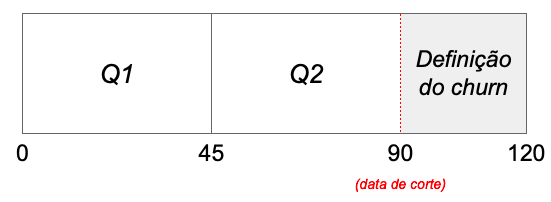
\includegraphics[scale=0.3]{quadrantes_desempenho.png}
    \end{figure}
\end{frame}

\begin{frame}
    \frametitle{Inclusão de outras covariáveis}
    \begin{itemize}
        \item Qualitativas
        \item Quantitativas "globais"
        \item Conjunto de dados final: 35 variáveis e 11131 observações
    \end{itemize}
\end{frame}

\begin{frame}
    \frametitle{Comparação dos modelos logísticos}
    \begin{itemize}
        \item Modelo 1: Stepwise (19 covariáveis)
        \item Modelo 2: LASSO (27 covariáveis)
        \item Modelo 3: LASSO + Stepwise (18 covariáveis)
        \item Escolhido o modelo 1 (teste da razão da verossimilhança)
    \end{itemize}
\end{frame}

\begin{frame}
    \frametitle{Diagnóstico e avaliação}
    \begin{itemize}
        \item Análise do comportamento dos resíduos quantílicos aleatorizados
        \item Análise da curva ROC (AUC: 0,89)
        \item Escolha do cutoff
        \item Sensibilidade: 0,84; Especificidade: 0,80
        \item Acurácia: 0,82 (IC: 0,80 - 0,84)
        \item Teste de concordância Kappa: 0,64
    \end{itemize}
\end{frame}

\begin{frame}
    \frametitle{}
    \centering Obrigado!
\end{frame}

\end{document}
